\documentclass[12pt,a4paper,onecolumn]{article}
\usepackage[pdfborder={0 0 0}]{hyperref}
\usepackage{amsfonts}
\usepackage{graphicx}
\usepackage{listings}
\usepackage{xcolor}
\usepackage{array}
\usepackage{enumitem}
\usepackage{longtable}
\usepackage{caption}

\begin{document}

\lstset{ %
  backgroundcolor=\color[rgb]{0.95,0.95,1.0},
  basicstyle=\footnotesize,        
  breakatwhitespace=false,         % sets if automatic breaks should only happen at whitespace
  breaklines=true,                 % sets automatic line breaking
  captionpos=b,                    % sets the caption-position to bottom
  commentstyle=\color[rgb]{0.3, 0.7, 0.3},    % comment style
  deletekeywords={...},            % if you want to delete keywords from the given language
  escapeinside={\%*}{*)},          % if you want to add LaTeX within your code
  extendedchars=true,              % lets you use non-ASCII characters; for 8-bits encodings only, does not work with UTF-8
  frame=single,                    % adds a frame around the code
  keepspaces=true,                 % keeps spaces in text, useful for keeping indentation of code (possibly needs columns=flexible)
  keywordstyle=\color{blue},       % keyword style
  language=C,                 % the language of the code
  morekeywords={*,...},            % if you want to add more keywords to the set
  numbers=none,                    % where to put the line-numbers; possible values are (none, left, right)
  numbersep=5pt,                   % how far the line-numbers are from the code
  numberstyle=\tiny\color{gray}, % the style that is used for the line-numbers
  rulecolor=\color{black},         % if not set, the frame-color may be changed on line-breaks within not-black text (e.g. comments (green here))
  showspaces=false,                % show spaces everywhere adding particular underscores; it overrides 'showstringspaces'
  showstringspaces=false,          % underline spaces within strings only
  showtabs=false,                  % show tabs within strings adding particular underscores
  stepnumber=2,                    % the step between two line-numbers. If it's 1, each line will be numbered
  stringstyle=\color[rgb]{0.58,0,0.82},     % string literal style
  tabsize=2,                       % sets default tabsize to 2 spaces
  title=\lstname                   % show the filename of files included with \lstinputlisting; also try caption instead of title
}

\begin{titlepage}
    \centering
    \vfill
    
\includegraphics[width=12cm]{EXOTica_clr.png}
    \vskip1cm
    {\bfseries\Huge
        The EXtensible Optimisation Toolset\\
        \vskip0.5cm
     \bfseries\Large
        EXOTica Acid (v 3.0.0)
        \vskip2.5cm
        Application Programming Interface
        \vskip1.5cm
     \bfseries\small
        Michael Camilleri
    }    
    \vfill
\end{titlepage}

\begin{abstract}
This document describes the Implementation of the EXOTica Library. The toolset aims to simplify the implementation of optimisation routines for robotic applications, particularly inverse-kinematics and path planning. The driving force behind the library is modularity (advocating a plugin architecture where users can re-implement individual components while making use of the rest) and re-usability.
\end{abstract}

\newpage
\tableofcontents

\newpage
\section{Introduction}
\label{INTRODUCTION}
This document describes the EXOTica library, a toolset for Kinematics and Dynamics optimisation problems for Robotic Systems. 

\subsection{Document Structure}
\begin{itemize}
\item General \textbf{Users} should read sections \ref{USING_THE_LIBRARY} and \ref{LIBRARY_IMPLEMENTATIONS}: optionally \ref{SETUP} is useful if they are new to ROS and the catkin build environment.
\item Those who wish to \textbf{extend} the library's functionality by adding new functionality should also read section \ref{EXTENDING_THE_LIBRARY}.
\item Finally \textbf{maintainers} should refer to the API section (\ref{MANAGING_THE_LIBRARY}, TODO) as well as the doxygen comments in the code.
\end{itemize}

\subsection{The EXOTica Library}
The EXOTica library is a generic Optimisation Tooolset for Robotics platforms, written in C++. It provides a framework for developing algorithms for Inverse-Kinematics and Trajectory Optimisation (and potentially Dynamic optimisation as well). Its design advocates:
\begin{itemize}
\item \textbf{Modularity} The library is developed in a modular manner making use of C++'s object-oriented features (e.g. polymorphism). This allows users to \textit{plug in} (mix'n match) different modules depending on their needs.
\item \textbf{Extensibility} The library is heavily extensible, mainly thanks to the modular design. In addition, the library makes very minimal prior assumptions about the form of the problem so that it can be as generic as possible. The end result is that users can work around the existing framework by \textit{extending} the library with new functionality to suit their needs, rather than \textit{rewriting} everything from scratch.
\item \textbf{Platform Independence} The toolset is designed to operate on a variety of robotic platforms, and as such is written with platform independence in mind. It is entirely OS-agnostic and the only library dependencies are Eigen and Boost. For ease of integration with the Robot Operating System (ROS), the build system is catkin but the library itself has no dependency on ROS and indeed, can be built using native compilers.
\item \textbf{Integration with ROS} Although it is not necessary, the library is fully integrate-able with ROS.
\end{itemize}

\newpage
\section{Setup}
\label{SETUP}

\subsection{Package Organisation}
EXOTica is currently organised in two (catkin) packages, plus an optional testing package.
\begin{itemize}
\item \textbf{exotica} contains the core library components and the abstract interface.
\item \textbf{exotations} (short for \textbf{exot}ica implement\textbf{ations}) holds the concrete implementations (currently Inverse-Kinematics) for the library.
\item \textbf{testing\_pkg} implements a series of automatic tests following the Google Test conventions.
\end{itemize}

\subsection{Pre-requisites}
The library currently has the following dependencies:
\begin{enumerate}
\item \textbf{Eigen} Library for matrix manipulation, specifically Eigen 3.0. Refer to http://eigen.tuxfamily.org/ for more information. Used throughout the library.
\item \textbf{Boost} to enforce thread-safety and prevent memory leaks. Please refer to http://www.boost.org/. Used throughout the library.
\item \textbf{Kinematica} for Kinematics problems (Forward and Inverse kinematics). A separate project by our group (http://wcms.inf.ed.ac.uk/ipab/slmc/research/EXOTica). Used by the \textit{IKTask} implementation.
\item \textbf{googletest} used within the testing package. Refer to https://code.google.com/p/googletest/.
\end{enumerate}
In addition, the testing package currently relies heavily on ROS (Hydro).


\subsection{Installation}
The current supported build system is Catkin from ROS: refer to the catkin tutorial at http://wiki.ros.org/catkin. One thing to note is that the library should be built using the C++11 compiler: this can be enforced by adding to the CMakeLists.txt:
\begin{verbatim}
set(CMAKE_CXX_FLAGS "${CMAKE_CXX_FLAGS} -std=c++0x")
\end{verbatim}

\noindent Alternatively, one may build the library (excluding the testing package) using another compiler: in this case, ensure that you link against the above libraries.

\newpage
\section{Introductory Optimisation Theory}
\label{OPTIMISATION_THEORY}
This section is a refresher of Optimisation problems and conventions. It aims to be as generic as possible, but wherever concrete examples are needed, reference is made to the task of solving Inverse Kinematics (IK).

\subsection{Notation}
Throughout this document we will use the following notation:
\begin{itemize}
\item Scalars will be represented by lower-case italic symbols ($x$).
\item Vectors are denoted by \textbf{bold} lower-case symbols ($\mathbf{x}$) indexed via a super-script ($\mathbf{x}^i$).
\item Matrices are denoted by \textbf{bold} UPPER-CASE symbols ($\mathbf{X}$) indexed by a double super-script ($\mathbf{X}^{i,j}$).
\item Time-domain indexing will be indicated by a subscript, as a function of $t$ (s.a. $x_{t-1}$): a discrete trajectory of $T$ steps is defined as a set of states from $t=0$ to $t=T-1$.
\item In contrast, a super-script $^T$ denotes a transpose.
\item A desired value for a state (such as a goal-state) is indicated by an asterisk ($x^*$).
\end{itemize}

\noindent In our setting, we describe a problem by Fig. \ref{FIG_PROBLEM_DESCRIPTION}:
\begin{figure}[!htp]
	\centering
    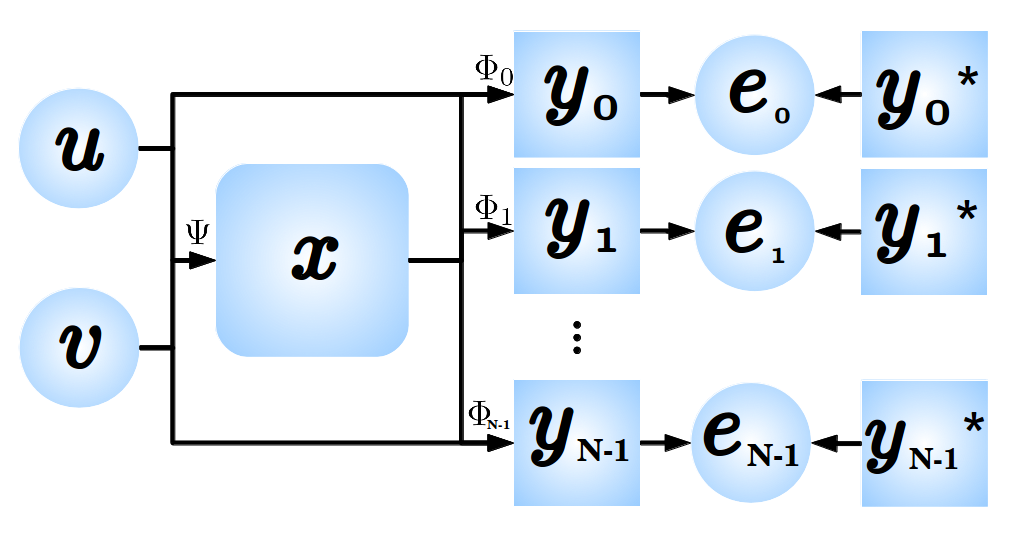
\includegraphics[width=0.85\textwidth]{Problem_description.png}
    \caption{Problem description within EXOTica}
   	\label{FIG_PROBLEM_DESCRIPTION}
\end{figure}\\

\noindent where we define:
\begin{itemize}
\item $\mathbf{u}$ : The Controllable inputs to the system (\textit{s.a. the changes in joint commands in IK}).
\item $\mathbf{w}$ : The External Uncontrolled inputs (\textit{such as the positions of obstacles}).
\item $\mathbf{q}$ : The \textbf{Configuration} of the system (\textit{for IK, this translates to simply the joint values}).
\item $\mathbf{x}$ : The State of the system, within the \textbf{Configuration} space: this could consist of $q$ and higher derivatives (typically with respect to time).
\item $\mathbf{y}$ : The Output(s) of the system, in \textbf{Task} space co-ordinates (\textit{s.a. position of end-effectors}). Note that we may have multiple different outputs.
\item $\mathbf{e}$ : An error/cost (defined below).
\item $\mathbf{\Psi}$ : The State-Transition function, mapping the evolution of the system through its dynamics/kinematics:
\begin{equation}
\mathbf{\dot x_{t+1}} = \Psi\left(\mathbf{x_t}, \mathbf{u_t}, \mathbf{w_t} \right) \label{EQ_STATE_TRANSITION_DEFINITION}
\end{equation}
\item $\mathbf{\Phi}$ : The Forward Mapping from the current configuration (state) to the task space: i.e.
\begin{equation}
\mathbf{y_t} = \mathbf{\Phi(x_{t}, u_t, w_t)} \label{EQ_PHI_DEFINITION}
\end{equation}
\end{itemize}

\subsection{Components}
Optimisation in Robotics usually involves defining a cost function around the system dynamics, which we then optimise, subject to certain constraints, to get the required commands \textbf{u} to apply to achieve our goals. Solution of such a function requires the following components.

\subsubsection*{Error Definition}
We represent our error, \textit{e}, through a function mapping from the desired and actual task-space co-ordinates to a \textbf{scalar} cost:
\begin{equation}
e_{t,i} = \mathbf{E_i}\left(\mathbf{y}_{t,i}, \mathbf{y}_{t,i}^*, \mathbf{C_i}\right) \label{EQ_ERROR_FUNCTION}
\end{equation}
where \textbf{C}$_i$ is a task-dependent cost matrix and \textbf{E}$_i$ is again indexed on the task.

\subsubsection*{Constraints}
Constraints impose limitations on the form the solution can take. Equality constraints are of the form:
\begin{equation}
\mathbf{f}\left(\mathbf{x}_t, \mathbf{\dot x}_{t+1}, \mathbf{u}_t, \mathbf{w}_t\right) = 0 \label{EQ_EQUALITY_CONSTRAINT}
\end{equation}
Similarly equality constraints, denoted by \textbf{g} are defined as:
\begin{equation}
\mathbf{g}\left(\mathbf{x}_t, \mathbf{\dot x}_{t+1}, \mathbf{u}_t, \mathbf{w}_t\right) > 0 \label{EQ_INEQUALITY_CONSTRAINT}
\end{equation}

\subsubsection*{Termination Criteria}
Termination Criteria are necessary when the solution requires iteration to converge: in this case, a termination criterion defines when a solution has been achieved and is represented by $\tau$. This maps the current state of the system to a binary true/false value.

\subsection{Cost Functions}
A generic time-dependent cost function as supported by EXOTica may seek optimisation over a number of simultaneous tasks, denoted \textit{0} through \textit{N-1}. There are multiple ways in which we can attempt to balance achieving them.

\subsubsection*{Weighted Optimisation}
One technique is to relatively weigh each task such that tasks with higher importance will be penalised more for deviation from the goal value. Eq.\ref{EQ_WEIGHTED_COST} is a generic representation of such a cost-function.
\begin{equation}
\mathbf{J} = \sum_{t=0}^{T-1}\sum_{i=0}^{N-1}\mathbf{\rho}_i e_{t,i} \label{EQ_WEIGHTED_COST}
\end{equation}
The outer summation is an iteration over the whole trajectory: since we are dealing with a numeric library, we ignore the case when this is continuous. The inner summation is over the tasks that define the problem. Finally $\rho$ denotes a scalar weighting factor between the individual tasks.

\subsubsection*{Prioritised Optimisation}
While allowing relative weighting between tasks/dimensions, Eq.\ref{EQ_WEIGHTED_COST} is still somewhat restrictive. In certain cases we may want a prioritised solution, meaning that a subset of goals are achieved, subject to first satisfying other goals. In this form, the higher-priority tasks appear as constraints to lower-priority ones. This is usually achieved through null-space resolution, whereby the solution of a task is cast into the null-space of those higher up and so on.

%\subsection{Optimisation}
%Optimisation of Eq.\ref{EQ_PRIORITISED_COST_FUNCTION} can proceed in a number of ways ranging from random Monte-Carlo like techniques to deterministic solutions. We present here one of the most common cases used, namely the Linear-Quadratic-Regulator (LQR) solver, for which the library is most suited: however, with some added effort, other techniques can also be used.
%
%\subsubsection*{Restrictions}
%In LQR, we restrict (or assume) that:
%\begin{enumerate}
%\item The forward mapping of the system is linear. In actual case we can usually approximate this for a small change in control inputs $\mathbf{\delta u}$:
%\begin{equation} \lim_{\delta u \rightarrow 0}\mathbf{\phi(u_t + \delta u)} = \mathbf{\phi(u_t)} + \mathbf{J(u_t)\delta u} \label{EQ_LQR_DYNAMICS}
%\end{equation}
%where we have dropped the implicit dependence of the function on the previous state ($\mathbf{x_t}$) and uncontrollable inputs ($\mathbf{v_t}$). In this case, \textbf{J}, referred to as the Jacobian, is the first derivative of the forward mapping $\mathbf{\phi}$, i.e.:
%\begin{equation}
%\mathbf{J}\left(\mathbf{u_t}\right) = \frac{\partial \mathbf{\phi}}{\partial \mathbf{u_t}} \label{EQ_JACOBIAN_DEFINITION}
%\end{equation}
%\item The cost functions, \textbf{f} and \textbf{g} are quadratic in nature, of the form:
%\begin{equation}
%h = ||\mathbf{z}^* - \mathbf{z}||_\mathbf{M} \label{EQ_LQR_COSTS}
%\end{equation}
%where \textbf{M} is the weighting matrix and \textbf{z} the task vector.
%\end{enumerate}
%
%\subsubsection*{The Solution}
%Optimisation of Eq.\ref{EQ_PRIORITISED_COST_FUNCTION} under the constraints imposed by \ref{EQ_LQR_DYNAMICS} and \ref{EQ_LQR_COSTS} results in the following deterministic solution:
%
%\begin{equation}
%\mathbf{u_t} = \mathbf{u_{t-1}} + \mathbf{J^\sharp}\left(\mathbf{y}^* - \mathbf{y}_{t-1}\right) + \left(\mathbf{I} - \mathbf{J^\sharp J} \right)\mathbf{h} \label{EQ_LQR_SOLUTION}
%\end{equation}
%\noindent where
%\begin{itemize}
%\item with a slight abuse of notation, the \textbf{y} here signifies the `\textbf{Big}' task-vector, which incorporates all the tasks at the same priority level.
%\item $\mathbf{J^\sharp}$ is the Jacobian pseudo-inverse, which depends on the task weighting matrices and regularisation matrices, besides the current configuration (for approximation of non-linear tasks). In effect, this is again the `\textbf{Big}' Jacobian, which incorporates all tasks at the same level.
%\item \textbf{h}, which is the null-space motion, is the solution (in input-space \textbf{u}) provided by tasks at a lower priority level. This is cast into the null-space of the current solution.
%\end{itemize}


\newpage
\section{Solving Optimisation Problems}
\label{USING_THE_LIBRARY}
This Section introduces the use of the library in as generic a way as possible, following the theory laid down in \ref{OPTIMISATION_THEORY}

\subsection{Architectural Overview}
EXOTica is implemented as a hierarchical structure, as displayed in Fig.\ref{FIG_EXOTICA_ARCHITECTURE}. 

\begin{figure}[!htp]
	\centering
    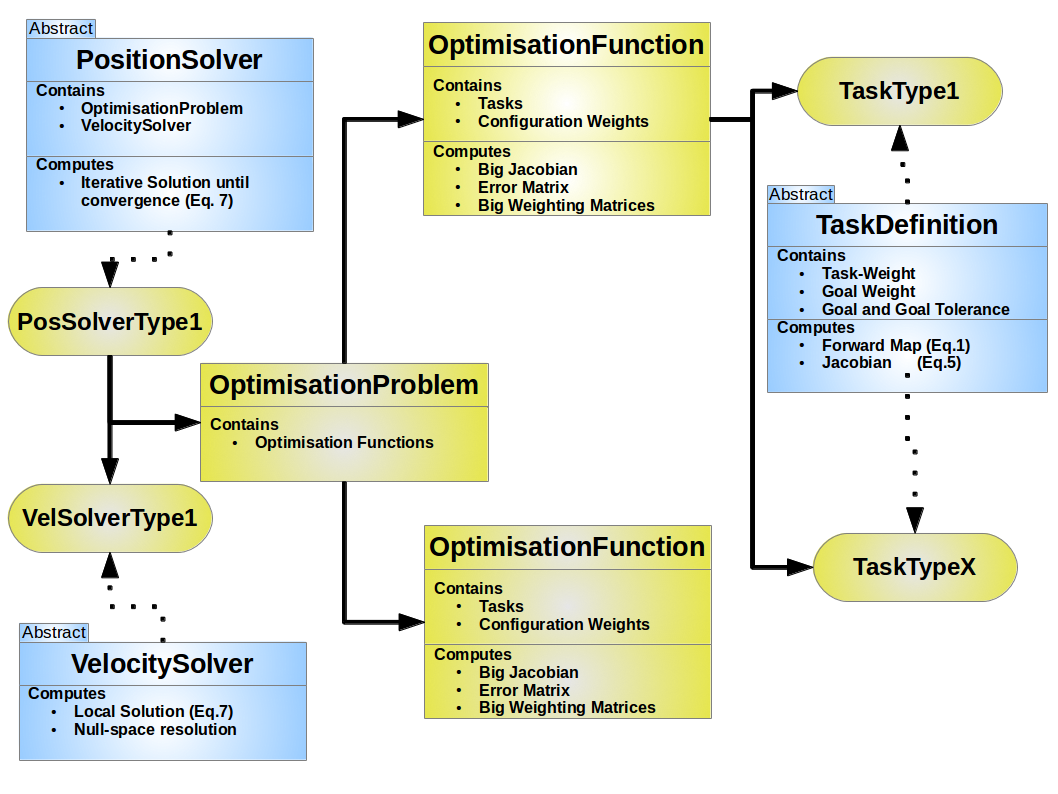
\includegraphics[width=\textwidth]{Exotica_Architecture.png}
    \caption{Architecture of the EXOTica library}
   	\label{FIG_EXOTICA_ARCHITECTURE}
\end{figure}


\noindent At the lowest level sits the abstract \textbf{TaskDefinition} object. This serves as a placeholder for the goal-vector (\textbf{y}$^*$), the goal weights ($\mathbf{W_n}$) and the inter-task weight ($\omega_n$). All concrete implementations inherit from it and implement at minimum specific computations for $\phi$ (Eq.\ref{EQ_PHI_DEFINITION}) and the Jacobian (Eq.\ref{EQ_JACOBIAN_DEFINITION}).\\
\newline
\noindent A set of tasks at the same priority level are encapsulated into an \textbf{OptimisationFunction} object. This provides a wrapper around a set of tasks at the same priority level (representing Eq.(\ref{EQ_WEIGHTED_COST_FUNCTION})). In turn, a hierarchy of Optimisation Functions is contained within an \textbf{OptimisationProblem}, by storing them in a user-defined order in an \textsl{std::vector}: in this case, the lower indices always have higher priority.\\
\newline
\noindent Finally, the solver is (usually) implemented in two stages:
\begin{itemize}
\item A \textbf{VelocitySolver} computes the incremental steps in converging towards the goal. It is also the responsibility of the velocity solver to resolve the priority levels and weightings of the problem. This amounts to computing the last two terms of Eq.(\ref{EQ_LQR_SOLUTION}).
\item The task of the \textbf{PositionSolver} is then to (possibly) iterate and integrate velocities until the solution converges.
\end{itemize}

\subsection{Boiler-Plate}
Generally, including the main header file is enough:
\begin{lstlisting} [belowskip=-1.5 \baselineskip]
#include <exotica/EXOTica.hpp>
\end{lstlisting}
Additionally, you may need to include implementation-specific headers for functionality which you implemented.\\
\newline
\noindent Using the library involves defining the Optimisation problem (basically Eq.(\ref{EQ_PRIORITISED_COST_FUNCTION})) and then solving. As an example, Inverse Kinematics will be used: we assume an implemented \textit{\textbf{IKTask}} together with \textit{\textbf{ISPosSolver}} and \textbf{\textit{ISVelSolver}} solvers\footnote{Implementation of these is indeed provided as part of the standard library.}.


\subsection{Initialisation}
The library currently provides two modes of initialisation, either through XML initialisation scripts or manually through setters and getters.

\subsubsection*{Initialisation through XML}
This is by far the easiest and preferred method for initialising the problem, since it takes care of everything, and also provides a great deal of flexibility. A symplified XML-file format appears below as Listing \ref{LISTING_XML_SIMPLIFIED}, while a more complete example for the IK-scenario is in the Appendix (Listing \ref{LISTING_XML_SPECIFICATION}).\\
\newline
\noindent The format is identified by the \textbf{Exotica} keyword, which must appear as the root element in every file (line 2). Its \textbf{only} children must be:
\begin{itemize}
\item The \textbf{OptimisationParamaters} : currently specifies only the window size of the trajectory (lines 3-5).
\item The \textbf{PositionSolver} definition (lines 7-35).
\end{itemize}
Note that these can however appear in any order.
\lstinputlisting[language=xml,
				keywordstyle=\color{blue}\bf,
				commentstyle=\color{blue},
				numbers=left,
    				numberstyle=\tiny,
    				numbersep=5pt,
    				stepnumber=1,
    				caption=Example XML-Specification,
    				label=LISTING_XML_SIMPLIFIED,
    				breaklines=true,
    				showstringspaces=false,
    				basicstyle=\footnotesize,
				stringstyle=\color{red},
				emph={Exotica,PositionSolver,OptimisationFunction,Task,
				      VelocitySolver,OptimisationParameters},
				emphstyle={\color{magenta}}]
				{simplified.xml}
The \textbf{PositionSolver} element encapsulates the complete problem. It may \textit{optionally} indicate use of a \textbf{VelocitySolver} (lines 8-10), which may in turn require specific parameters. In both cases the \textit{type} of solver(s) must be specified as an attribute. The \textbf{PositionSolver} element should also contain reference to a \textit{single} \textbf{OptimisationFunction}, which is optionally named. This element defines the actual problem (lines 12-34). It contains the matrix of configuration weights (line 13)\footnote{Note that matrix definitions require a \textbf{dim}ension attribute and should be listed in row-major order.} and \textit{at least} one \textbf{Task} (lines 15-24).\\
\newline
\noindent The \textbf{Task} contains reference to the universal task-parameters (goal-weights, goal, tolerance, inter-task weighting) organised as an \textit{ordered} list of \textbf{TimeElement}s, one for each time-step of the trajectory (whose size must equal the Window parameter). In additional specific implementations may require additional parameters which must also be specified, but outside the \textbf{TaskParameters} tag.\\
\newline
\noindent If a priority scheme is required, this is indicated by a nested \textbf{OptimisationFunction} element, which may in turn contain other such elements for a complex nesting problem.\\
\newline
\noindent One final thing to note is that in general the order in which elements appear is irrelevant except for:
\begin{itemize}
\item The Order of nesting of \textbf{OptimisationFunction}s defines the null-space priority resolution
\item The Order of \textbf{TimeElement}s within the \textbf{Task} is associated with the parameters at each time-step of the trajectory.
\end{itemize}
\noindent Once the XML-specification is defined, EXOTica provides an initialiser function which does all the work for you.
\begin{lstlisting}[belowskip=-1.5 \baselineskip, numbers=left]
boost::shared_ptr<exotica::PositionSolver>  pos_solv_ptr;
tinyxml2::XMLDocument                       document;

if (document.LoadFile("path_to_spec") == tinyxml2::XML_NO_ERROR)
{
	tinyxml2::XMLHandle xml_handle(document);
	if (exotica::initialiseSolver(xml_handle, pos_solv_ptr_))
	{
		//!< Execute
	}
}
\end{lstlisting}
The above code creates a Boost smart pointer to a \textbf{PositionSolver} object and then attempts to load the XML specification (checking that it is correctly formatted in the process). The \textit{\textbf{initialiseSolver(...)}} function in turn, takes an XMLHandle and the shared pointer in which to store the solver. It return true if everything is successful and false otherwise.

\subsubsection*{Manual Initialisation}

Coming Soon

%\begin{lstlisting} [belowskip=-1.5 \baselineskip]
%exotica::OptimisationFunction optim_func; //!< My optimisation function
%  Eigen::VectorXd config_weights = Eigen::VectorXd::Ones(dimension_)*1e-3;//Set R
%  std::string optim_name = "pos_IK"; //Set Name
%  optim_func.setParams(&optim_name, &config_weights); //by Pointer
%\end{lstlisting}
%
%\noindent The name member is merely for convenience, while the regularisation weights are taken to be equal and quite small. Note that in the current implementation, these must be passed via pointers (allowing the user to specify NULL and thus keep the internal value unchanged), which is why we had to create the variables outside the function call.\\
%\newline
%\noindent The task can now be defined using the \textit{\textbf{add\_task(...)}} method:\\
%\newline
%\begin{lstlisting} [belowskip=-1.5 \baselineskip]
%if (optim_func.addTask("IKTask", "position", exotica::default_params) != True)
%{
%	cout << "Oops! Unable to create task of type IKTask" << endl;
%	return;
%}
%\end{lstlisting}
%This function takes in three parameters:
%\begin{enumerate}
%\item The Type of the Task, identified by its name. In EXOTica, each Task implementation has a unique name. Refer to Section \ref{LIBRARY_IMPLEMENTATIONS} for a list of Tasks within the standard library.
%\item The name that we will use to access this task: this can be any unique string.
%\item The Optimisation Parameters. These are optimisation-wide parameters, which currently (in EXOTica v1.0.0) consist of:
%\begin{itemize}
%\item \textbf{optimisation\_window} : the size of the trajectory over which to optimise: for the IK task this is by definition unity.
%\item \textbf{max\_iter} : The maximum number of iterations when searching for a solution.
%\item \textbf{max\_step} : The maximum step size to interpolate over at every iteration (for a complete optimisation cycle). A negative value indicates there should be no scaling.
%\end{itemize}
%\end{enumerate}
%\noindent \textit{default\_params} is a static instantiation of the above structure with a window size of 1, 20 maximum iterations and a step-size of 0.002. Otherwise, it can be defined as necessary.\\
%\newline
%\noindent In addition each task needs values for the intra- and inter-task weights. Access to the task is through a \textbf{\textit{boost::weak\_ptr}} to enforce thread-safety.
%
%\begin{lstlisting}
%{
%	boost::shared_ptr<exotica::IKTask> task_ptr = boost::dynamic_pointer_cast<exotica::IKTask> (optim_func.access("position").lock());
%	if (task_ptr.get() != nullptr) {
%		if (!task_ptr->setGoalWeights(Eigen::MatrixXd::Identity(3,3))) { return false; } //All goals equal priority
%		if (!task_ptr->setTaskWeight(1.0)) { return false; } //Fail
%	}
%}	
%\end{lstlisting}
%\noindent Note how the operations are carried out within a new block to enforce locality of the task\_ptr. Additionally, different tasks may require additional parameters, specific to the implementation, and should be set at this point (again refer to section \ref{LIBRARY_IMPLEMENTATIONS} for specifics).\\
%\newline
%\noindent Once this is fully initialised, it can be pushed back into a vector\footnote{Here we use the C++11 initialiser list format.}:
%\begin{lstlisting}
%std::vector<exotica::OptimisationFunction> my_optimisation = {optim_func};
%\end{lstlisting}
%
%\noindent Similarly, an orientation task definition can be defined and pushed back to the vector. Note that although the ordering of tasks within a single optimisation function does not matter (i.e. it does not depend on the order in which \textbf{\textit{addTask(...)}} is called), the order of optimisation functions within the optimisation vector does, as this represents the priority level!

\subsection{Solving the Optimisation Problem}

Coming Soon
%Once the task is defined, the solution can proceed. We first need to instantiate a position solver and velocity solver:
%
%\begin{lstlisting} [belowskip=-1.5 \baselineskip]
%boost::shared_ptr<exotica::ISPosSolver> ik_pos(new exotica::ISPosSolver(default_params));
%boost::shared_ptr<exotica::ISVelSolver> ik_vel(new exotica::ISVelSolver(default_params));
%\end{lstlisting}
%There are a few things to note:
%\begin{itemize}
%\item Both solvers are initialised from the same value of optimisation parameters. This is important for correct functioning of the library.
%\item A shared pointer of each object is instantiated. This is necessary \textbf{only} for the velocity solver, for reasons which will become clear below.
%\end{itemize}
%Depending on the type of solvers, additional parameters may need to be set: please refer to the appropriate documentation.\\
%\newline
%\noindent The final step is to call the \textbf{\textit{solve(...)}} function:
%
%\begin{lstlisting}
%Eigen::VectorXd joint_solution;
%
%if (!ik_pos.solve(my_optimisation, Eigen::VectorXd::Zeros(7), &ik_vel, joint_solution)) { return false; }
%\end{lstlisting}
%The function takes four arguments:
%\begin{enumerate}
%\item The vector of optimisation functions
%\item The initial configuration
%\item Shared Pointer to the velocity solver: this is required to allow for polymorphism of inherited velocity solver implementations\footnote{This is also the reason why the velocity solver was created through a shared pointer in the first place. It is important that this is so, because if we just pass the address of a stack-variable, it will try to delete the memory after the function exits which is illegal given that the variable would not have been dynamically allocated.}.
%\item The vector where to store the configuration-solution.
%\end{enumerate}
%
%\noindent Again, once the solution is achieved, a new goal may be set and solutions queried once more. The library is optimised such that data reuse improves efficiency (most often, we do no need to change weightings/task specifications between queries).

\newpage
\section{Library Implementations}
\label{LIBRARY_IMPLEMENTATIONS}
This section lists a number of implementations which come bundled as part of the standard library, with Tasks, Velocity and Position solvers being listed independently. As much as possible, these modules are interchangeable and indicated if this is not so. Information on general usage is provided, together with dependencies (outside exotica) and initialisation details. Refer to the appropriate documentation for more details.

\subsection{Task Definitions}
Task Definitions are defined hereunder. The unique string identifier is given in bold blue.\\

\begin{longtable}{p{3cm}p{10cm}}
\textbf{\textcolor{blue}{IKTask}} & \textit{\textbf{I}nverse-\textbf{K}inematics \textbf{Task}}\\
\hline \\
\textbf{Class:} & ex\_ik/IKTask \\
\textbf{Description:} & Implements Positional Inverse Kinematics based on Geometric Jacobian for arbitrary robot end-effectors. \\
\textbf{Dependencies:} &  Kinematica \\
\textbf{Initialisation:} & Two signatures, one taking a urdf file and another a pre-initialised KDL::Tree, together with a set of Solution parameters: refer to the Kinematica Documentation. Both return indication of Success/Failure (True/False respectively). \begin{lstlisting} [belowskip=-2.5 \baselineskip]
bool initTask(const std::string &, const kinematica::SolutionForm_t)
bool initTask(const KDL::Tree &, const kinematica::SolutionForm_t)
\end{lstlisting} \\
\textbf{Notes:} & By definition an IK-Task only defines a single-time solution (initialisation parameters are ignored).
\end{longtable}

\newpage
\subsection{Velocity Solvers}
These are the velocity solvers which are currently implemented.\\

\begin{longtable}{p{3cm}p{10cm}}
\textbf{\textcolor{blue}{ISVelSolver}} & \textit{\textbf{I}terative \textbf{S}ingle-point \textbf{Vel}ocity \textbf{Solver}}\\
\hline \\
\textbf{Class:} & ex\_iss/ISVelSolver \\
\textbf{Description:} & Implements a velocity solver for one-shot trajectories (although may iterate to achieve at solution). Uses the Moore-Penrose pseudo-inverse. \\
\textbf{Dependencies:} &  None \\
\textbf{Initialisation:} & Need to set the inverse format through:
\begin{lstlisting} [belowskip=-1.0 \baselineskip]
void setPinvMode(ISVel_pinv_t)
\end{lstlisting} The Parameter can take on three values:
\begin{itemize} 
\item IS\_PI\_LEFT : Use the Left Pseudo-Inverse ($J^TWJ+R)^{-1}J^TW$)
\item IS\_PI\_RIGHT : Use the Right Pseudo-Inverse ($W^{-1}J^T(JR^{-1}J^T+W^{-1})^{-1}$)
\item IS\_PI\_AUTO : Let the solver decide based on numerical stability.
\end{itemize}\\
\textbf{Notes:} & Since this is a one-shot solver, indexing parameters are ignored.
\end{longtable}

\newpage
\subsection{Position Solvers}
These are the velocity solvers which are currently implemented.\\

\begin{longtable}{p{3cm}p{10cm}}
\textbf{\textcolor{blue}{ISPosSolver}} & \textit{\textbf{I}terative \textbf{S}ingle-point \textbf{Pos}ition \textbf{Solver}}\\
\hline \\
\textbf{Class:} & ex\_iss/ISPosSolver \\
\textbf{Description:} & Implements a position solver for one-shot trajectories, but iterates over the solution until convergence. Uses a Newton-Raphson style of search, but scales down intermediate velocity solutions to avoid instabilities. \\
\textbf{Dependencies:} &  None \\
\textbf{Initialisation:} & Default \\
\textbf{Notes:} & Since this is a single-position solver, it does not use the index value. \\
\end{longtable}


\newpage
\section{Extending the Library}
\label{EXTENDING_THE_LIBRARY}
One of the major goals of this project is to provide an extendible platform. This applies both at the level of task-types, velocity solvers and position solvers. Hence, implementing any of these abstract classes allows the library to grow as required.

\subsection{Creating Task-Definition Classes}
The TaskDefinition class \textbf{must} contain everything that defines the task. This is currently an abstract interface and must be implemented to model the required problem (for example an IK-type task).
\subsubsection*{The Abstract Interface}
The abstract class itself handles storage of the weighting matrix for intra-task weights, the inter-task weights as well as the goal vector (with tolerance). In addition, it provides support for trajectory optimisation and hence deals with vectors of the above data structures, one for each time-step (by default the vector is of size 1).  Finally, the base-class as it is is guaranteed to be thread-safe.
\subsubsection*{Inheriting from the TaskDefinition Class}
All inherited objects must implement two pure-virtual functions:
\begin{lstlisting} [belowskip=-1.0 \baselineskip]
bool updateState(const Eigen::VectorXd &, int)
bool initDerived(tinyxml2::XMLHandle &)
\end{lstlisting}
The first function takes as inputs the vector of current configuration and the index into the trajectory vector. Ideally the latter parameter should default to 0. The function should:
\begin{enumerate}
\item Compute the Forward mapping, given the current configuration and store it in the appropriate phi-matrix (use the \textbf{\textit{setPhi(..)}} method).
\item Compute the Jacobian and store it in the appropriate Jacobian matrix (use the \textbf{\textit{setJacobian(...)}} method).
\item Indicate whether all computations were successful (True) or not (False) through the return value.
\end{enumerate}
The second function is used to initialise any implementation-specific parameters for the task. If it is not required, it should only return true.

\subsubsection*{Registering the Task}
In order to allow dynamic instantiation of the inherited classes through the \textbf{\textit{OptimisationFunction::addTask(...)}} method, the library uses object factories. These however must be provided with knowledge of the inherited classes itself. A macro is provided for this:
\begin{lstlisting} [belowskip=-1.0 \baselineskip]
REGISTER_TASK_TYPE ("TaskName", TaskType) 
\end{lstlisting}
The first parameter must be a \textbf{unique} string identifier which users will use to refer to the class. The second is the actual class name. This line must appear within the class implementation file (\textit{*.cpp}) and \textbf{not} the header file.
\subsubsection*{Tips and Tricks}
\begin{itemize}
\item Ideally, (unless it is irrelevant such as for IK) support for multi-point trajectory optimisation should be maintained through the use of vectors for all parameters.
\item Enforce thread-safety through mutexes. This is a major requirement of this object. One efficient way of dealing with the fact that the jacobian computation typically calls the forward map function is to have the forward map call a \textbf{private} unlocked compute function which is also the function used by the jacobian computer. All public interfaces will be blocking but this internal one will not so there won't be a problem due to blocking within the same thread.
\item Ideally, since the classes can be instantiated dynamically, it is preferable to check for correct initialisation within the \textit{compute} functions.
\item Ideally, inherited objects should use default arguments for the index variable to ease implementation of single-point trajectories.
\end{itemize}

\subsection{Creating Position Solvers}
Position Solvers define the interpolation and approximation process in solving optimisation problems by interpolating velocity changes. The class is currently an Abstract Interface.
\subsubsection*{The Abstract Interface}
The PositionSolver abstract class only holds the optimisation parameters and that is it.
\subsubsection*{Inheriting from the PositionSolver class}
All inherited objects must implement the solve function:
\begin{lstlisting} [belowskip=-1.25 \baselineskip]
bool solve(std::vector<OptimisationFunction> &, const Eigen::VectorXd &, boost::shared_ptr<VelocitySolver>, Eigen::VectorXd &)
\end{lstlisting}
The inputs are in order:
\begin{enumerate}
\item Vector of Optimisation Functions
\item Initial Configuration of the robot
\item Shared Pointer to the Velocity Solver: the reason for this is to allow polymorphic use of different velocity solvers.
\item Configuration vector for the solution
\end{enumerate}
Ideally it should indicate success or failure through the return variable: note however that this success/failure is only at the level of computation and should \textbf{not} indicate whether the goal was reached or not. The function is intended to call the velocity solver's \textbf{\textit{solve()}} function for actually computing incremental updates to the current solution: it is thus the task of the position solver to integrate these local solutions to achieve a final result.

\subsubsection*{Tips and Tricks}
\begin{itemize}
\item Again, ensure that thread safety is maintained as much as possible within the \textit{\textbf{solve(...)}} function.
\item The position and velocity solvers are tightly coupled although they are still independent. Take care of this in implementation.
\item In the interest of efficiency, it was decided to put the responsibility of updating the task variables within the Position Solver rather than the Velocity Solver object. In fact, the only communication to the velocity solver is the optimisation function which must be completely defined. Specifically, the position solver should call the \textbf{\textit{updateTask()}} on the optimisation function before calling on the Velocity Solver.
\end{itemize}

\subsection{Creating Velocity Solvers}
The final piece of the puzzle is the velocity solver which computes "locally approximate velocities" to reduce the error towards the goal. The class is also an abstract interface.
\subsubsection*{The Abstract Interface}
The Abstract version of the class serves as a place-holder for the optimisation parameters (which must be initialised through the constructor). It exposes two functions, one to solve for the optimal velocity which in turn calls the inverse-calculator. In the interest of modularity, both may be overloaded, but the inverse-function is pure-virtual and so \textbf{must} be implemented. A default implementation is provided for the \textbf{solve} function to handle the construction of the weight matrices for passing on to the pseudo-inverse calculation, as well as the casting of temporary solutions into the null-spaces required:
\begin{lstlisting}[belowskip=-1.0 \baselineskip]
bool solve(std::vector<OptimisationFunction> &, Eigen::VectorXd &, int=0)
\end{lstlisting}
with parameters:
\begin{enumerate}
\item The Vector of optimisation functions (pre-initialised and updated).
\item Placeholder for the resulting \textbf{velocity vector}.
\item Integer index: defaults to 0.
\end{enumerate}
\subsubsection*{Inheriting from the VelocitySolver class}
All classes inheriting from the velocity solver \textbf{must} implement the inverse computation:
\begin{lstlisting} [belowskip=-1.25 \baselineskip]
bool getInverse(const Eigen::MatrixXd &, const Eigen::MatrixXd &, const Eigen::MatrixXd &, Eigen::MatrixXd &)
\end{lstlisting}
The function takes the following arguments (in order):
\begin{enumerate}
\item The `\textbf{big}' \textbf{Jacobian} to invert.
\item The \textbf{Configuration-Weight Matrix} $R$.
\item The `\textbf{big}' \textbf{Task-Weight Matrix} $W$.
\item The place-holder for the resulting inverted \textbf{Jacobian}.
\end{enumerate}
In keeping with the convention of the library, it should indicate success or failure of the solution. Typically, the pseudo-inverse can take the form of the moore-penrose decomposition or singular value decomposition, but this is entirely up to the implementer.\\
\\
\noindent Additionally, one may choose to overload the solve function, although this is not necessary.
\subsubsection*{Tips and Tricks}
\begin{itemize}
\item It is important that the \textbf{\textit{getInverse(...)}} function indicates success through its return value, as this is checked by the \textbf{\textit{solve(...)}} function. At the very least it should always return true.
\item While it might be a bit tricky, thread-safety should be encouraged throughout the implementation.
\end{itemize}


\newpage
\section{Detailed API}
\label{MANAGING_THE_LIBRARY}
For this version of documentation, the reader is asked to refer to the in-code documentation (particularly comments in the header files) for detailed information. Future releases will contain a separate section with the full API.

%\subsection{The Task Definition Class}
%\subsection{The Task Factory}
%\subsection{The Optimisation Function Class}
%\subsection{The Position Solver Class}
%\subsection{The Velocity Solver Class}
%\subsection{Miscellenaous}

\newpage
\appendix
\section{Limitations}
\begin{itemize}
\item Currently, there is no object-factory concept for the position/velocity solvers
\item Initialising Optimisation Functions is still pretty painful.
\end{itemize}
\section{Version History}


	\begin{longtable}{|m{2.0cm}||m{6cm}|m{6cm}|}
	\hline
	\textbf{Version} & \textbf{Library Changes} &  \textbf{Documentation Changes}\\
	\hline
	\hline
	\center{\textbf{0.0.1}} & \begin{itemize}[leftmargin=0.35cm] 
	\item First Iteration of EXOTica
	\end{itemize}
				  & \begin{itemize}[leftmargin=0.35cm]
				    \item First Documentation
				  	\end{itemize}\\
	\hline	
	\center{\textbf{1.0.0 (Venom)}} & \begin{itemize}[leftmargin=0.35cm]
					\item First Official Release
					\item Changed API for updating the Task state to a single function rather than individually for the Jacobian/Forward Map.
					\item Fixed bug with calling setter functions on uninitialised vector of task parameters.
					\item In the interest of efficiency, state updating was moved to the PositionSolver: hence the configuration variable for the VelocitySolver was removed.
					\end{itemize} & \begin{itemize}[leftmargin=0.35cm]
				    \item Changed Sections \ref{USING_THE_LIBRARY} and \ref{EXTENDING_THE_LIBRARY}.
				    \item Added Section \ref{LIBRARY_IMPLEMENTATIONS} on specific implementations.
				  	\end{itemize} \\
	\hline
	\center{\textbf{1.0.0 (Venom)}} &
					\begin{itemize}[leftmargin=0.35cm]
					\item Moved initialisation of optimisation parameters to within an initialiser constructor and removed default constructor. However, the create function has a default argument for the window (being 1). Similarly modified the \textbf{\textit{OptimisationFunction::addTask()}} to reflect this, however, without default parameters. There is however a default initialisation for the \textit{OptimisationParameters\_t} (a \textbf{const static} instantiation called \textbf{\textit{default\_params}})
					\item Added function to get configuration dimension to the OptimisationFunction class. Also changed internal storage of configuration weights to be matrix rather than vector.
					\item Fixed bug whereby when checking the dimensionality of the configuration or task space I was asking for \textbf{\textit{size()}} rather than \textbf{\textit{rows()}} in a 2D matrix.
					\item Fixed bug in computation of task error within the \textit{OptimisationFunction} class.
					\end{itemize} & \\
	\hline
	\center{\textbf{2.0.0 (Kinky Slinky)}} &
					\begin{itemize}[leftmargin=0.35cm]
					\item Completely re-organised the architecture of the library with respect to containment.
					\item Created the OptimisationProblem wrapper around the vector of OptimisationFunctions.
					\item Implemented XML-based initialisation for all classes.
					\item Added factories for the Position and Velocity Solvers.
					\item Added JointLimits Task (not documented yet).
					\item Extensively tested.
					\end{itemize} & \begin{itemize} [leftmargin=0.35cm]
					\item Partially modified documentation (wip).
					\end{itemize} \\
	\hline	
	\end{longtable}
	
\newpage
\section{Listings}
\lstinputlisting[language=xml,
				keywordstyle=\color{blue}\bf,
				commentstyle=\color{blue},
				numbers=left,
    				numberstyle=\tiny,
    				numbersep=5pt,
    				caption=Example XML-Specification,
    				label=LISTING_XML_SPECIFICATION,
    				breaklines=true,
    				showstringspaces=false,
    				basicstyle=\footnotesize,
				stringstyle=\color{red},
				emph={Exotica,PositionSolver,OptimisationFunction,Task,
				      VelocitySolver,OptimisationParameters},
				emphstyle={\color{magenta}}]
				{specification.xml}

\end{document}